%!TEX root = ../thesis.tex

\section{学習フェーズ}

  学習フェーズのシステムを\figref{Fig:RobotGuidance_learning_system}に示す.このフェーズでは,ルールベース制御器を用いてロボットを制御する.ルールベース制御器は,反射強度の高い方向にロボットを追従させる制御で,\figref{Fig:RobotGuidance_learning_phase_leg}に示すように,追従対象者に再帰反射テープを装着し,2DLiDARでそれを検出することで,ロボットが人に追従する.このとき,入力は2DLiDARの反射強度であり,出力はロボットのヨ―方向の角速度$\omega$となる.並行して,この行動とカメラの画像データを深層学習器に入力して,オンラインでend-to-end学習する.

  \vspace{0.5cm}

  \begin{figure}[h]
    \centering
    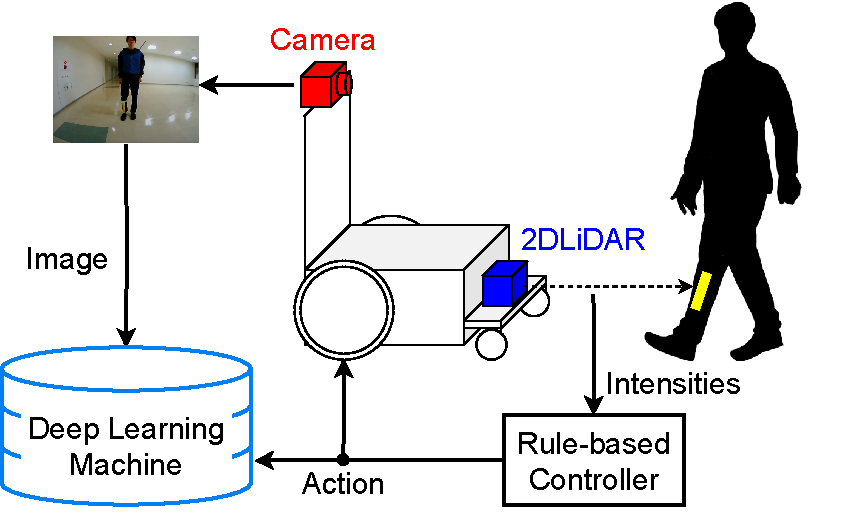
\includegraphics[width=9cm] {images/pdf/RobotGuidance_learning_system}
    \captionsetup{justification=raggedright} % キャプションを左寄せに
    \caption{System in the learning phase}
    \label{Fig:RobotGuidance_learning_system}
  \end{figure}

  \vspace{0.5cm}

  \begin{figure}[h]
    \centering
    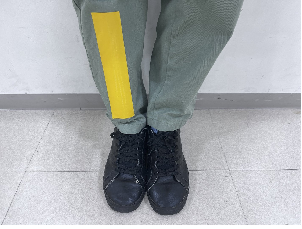
\includegraphics[width=4.5cm] {images/pdf/RobotGuidance_learning_phase_leg}
    \captionsetup{justification=raggedright} % キャプションを左寄せに
    \caption{Attachment retroreflective tape}
    \label{Fig:RobotGuidance_learning_phase_leg}
  \end{figure}

\newpage
